\documentclass[a4paper, 11pt]{article}
\usepackage{geometry}
\geometry{letterpaper, margin=1in}
\usepackage{amsmath}
\usepackage{amssymb}  
\usepackage{amsthm}
\usepackage{ulem} 
\usepackage{graphicx}
\usepackage{physics}
\graphicspath{ {images/} }

\begin{document}
%Header-Make sure you update this information!!!!
\noindent
\large\textbf{Complex Analysis: Assignment 1} \hfill \textbf{John Waczak} \\
\normalsize MTH 483 \hfill  Date: \today \\

\section*{1.1abc}
Let $z = 1 + 2i$ and $w = 2 -i$. Compute the following: \\

\noindent(a) $z + 3w$ \\ 
	\begin{align*}
		z+3w &= (1+2i)+3(2-i)\\
			&= 1+6+2i-3i \\ 
			&= 7-i
	\end{align*}

\noindent(b) $\overline{w}-z$
	\begin{align*}
		\overline{w}-z &= (2-i)^*-(1+2i) \\ 
			&= (2+i)-(1+2i) \\
			&= 2+i-1-2i \\ 
			&= 1-i
	\end{align*}
	
\noindent(c) $z^3$
	\begin{align*}
		z^3 &= (1+2i)^3 \\
			&= (1+2i)(1+2i)(1+2i) \\ 
			&= (1+2i)(-3+4i) \\ 
			&= -3-6i+4i-8 \\ 
			&= -11 -2i
	\end{align*}
	
\section*{1.2ab}
Find the real and imaginary parts of the following:\\

\noindent(a) $\frac{z-a}{z+a}$ with $a\in\mathbb{R}$ \\ 

let $z = x + iy$. Then: 	
	\begin{align*}
		\frac{z-a}{z+a} &= \frac{x+iy-a}{x+iy+a} \\ 
			&= \frac{(x-a)+iy}{(x+a)+iy} \\ 
			&= \frac{[(x-a)+iy][(x+a)-iy]}{(x+a)^2+y^2} \\ 
			&= \frac{x^2+a^2+y^2+2ayi}{(x+a)^2+y^2} 
	\end{align*}
 Thus identifying the imaginary and real parts gives:
	 \begin{align*}
	 	\Re\Big(\frac{z-a}{z+a}\Big) &= \frac{\Re(z)^2+a^2+\Im(z)^2}{(\Re(z)+a)^2+\Im(z)^2} \\ 
	 	\Im\Big(\frac{z-a}{z+a}\Big) &= \frac{2a\Im(z)}{(\Re(z)+a)^2+\Im(z)^2}
	 \end{align*}
	
\noindent(b) $z= \frac{3+5i}{7i+1}$
	\begin{align*}
		\frac{3+5i}{7i+1} &= \frac{3+5i}{1+7i} \frac{1-7i}{1-7i} \\ 
			&= \frac{(3+5i)(1-7i)}{1+49} \\ 
			&= \frac{1}{50}(38 - 16i) \\
			&= \frac{19}{25}-\frac{8i}{25}
	\end{align*} 
	\begin{align*}
		\text{thus: }\Re(z) &= \frac{19}{25} \\ 
		\Im(z) &= -\frac{8}{25} 
	\end{align*}	
	
\section*{1.3abd}
Find the absolute value and conjugate of the following: \\ 

\noindent(a) $z = -2+i$
	\begin{align*}
		|z| &= |-2+i| \\ 
			&= \sqrt{4+1} \\ 
			&= \sqrt{5} \\
		\overline{z} &= -2-i
	\end{align*}
	
\noindent(b) $z=(2+i)(4+3i)$ 
	\begin{align*}
		z &= 8-3+4i+6i \\ 
			&= 5+10i \\
		\Rightarrow |z| &= \sqrt{125} = 5\sqrt{5} \\ 
		\overline{z} &= 5-10i
	\end{align*}	
	
\noindent(d) $z=(1+i)^6$ 
	\begin{align*}
		z &= (\sqrt{2})^6\Big(\frac{\sqrt{2}}{2}+\frac{\sqrt{2}}{2}i\Big)^6 \\ 
			&= (\sqrt{2})^6(e^{i\pi/4})^6 \\ 
			&= 2^3e^{i3\pi/2} \\ 
			&= 8e^{i3\pi/2} \\
			&= -8i \\
		\Rightarrow |z| &= 8 \\ 
		\text{and} \quad	\overline{z} &= -8i 	
	\end{align*} 
	
	
\section*{1.4ace}
Write the following in polar form.\\

\noindent(a) $z=2i$ 
	\begin{align*}
		z &= 2i = 2e^{i\pi/2} \\ 
	\end{align*}
	
\noindent(c) $z=-3+\sqrt{3}i$ 
	\begin{align*}
		r &= \sqrt{9+3} = \sqrt{12} = 2\sqrt{3} \\ 
		\Rightarrow 2\sqrt{3}\cos\theta &= -3 \\ 
			\cos\theta &= -\frac{\sqrt{3}}{2} \\ 
		\text{and} \quad 2\sqrt{3}\sin\theta &= \sqrt{3} \\ 
			\sin\theta &= \frac{1}{2}\\ 
		\Rightarrow \theta &= 5\pi/6 \\ 
		\text{thus} \quad  z &= 2\sqrt{3}e^{i5\pi/6}
	\end{align*}

\noindent(e) $z = (2-i)^2$ 
	\begin{align*}
		\text{first}\quad 2-i &\Rightarrow r = \sqrt{5} \\ 
			\theta &= \arctan(-1/2) \\ 
		\text{thus }\quad z &= (\sqrt{5}e^{i\arctan(-1/2)})^2 \\ 
			&= 5e^{2i\arctan(-1/2)}
	\end{align*}
	
\section*{1.5ab}
Write the following in their Cartesian representation.\\

\noindent(a) $z=\sqrt{2}e^{i3\pi/4}$
	\begin{align*}
		z &=\sqrt{2}e^{i3\pi/4} \\
			&= \sqrt{2}\cos(3\pi/4)+i\sqrt{2}\sin(3\pi/4) \\ 
			&= -\sqrt{2}\frac{\sqrt{2}}{2}+i\sqrt{2}\frac{\sqrt{2}}{2} \\ 
			&= -1+i
	\end{align*}
	
\noindent(b) $z = 34e^{i\pi/2}$ 
	\begin{align*}
		z &= 34\cos\pi/2 + i34\sin\pi/2 = 34i 
	\end{align*}

\section*{1.8b}
Use the quadratic formula to solve the following. \\

\noindent(b) $2z^2+2z+5=0$ 
	\begin{align*}
		z &= \frac{-2 \pm \sqrt{4-4\cdot2\cdot5}}{2\cdot2} \\ 
			&= \frac{-2 \pm \sqrt{-36}}{4} \\ 
			&=\frac{-2 \pm 6i}{4} \\ 
			&= -\frac{1}{2} \pm \frac{3}{2}i
	\end{align*}
	
\section*{1.11bc} 
Find all solutions to the following equations:\\

\noindent(b) $z^4 = -16$ \\ 
	\begin{align*}
		z^4 &= 16e^{i(\pi + 2\pi n)}\\ 
		z	&= 16^{1/4}e^{i(\pi/4+n\pi/2)} \quad n\in[0, 1, 2, 3] \\ 
			&= 2e^{i(\pi/4+n\pi/2)}\\
			&= \big\{ 2e^{i\pi/4}, 2e^{i3\pi/4}, 2e^{i5\pi/4}, 2e^{i7\pi/4} \big\}
	\end{align*}
\pagebreak
These roots form a regular square
	\begin{figure}[!hbt]
		\centering
		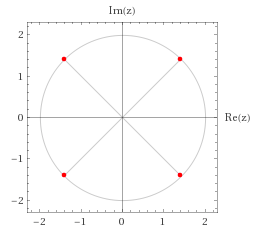
\includegraphics[scale=0.75]{fourthRoots}
	\end{figure}
	
\noindent(c) $z^6 = -9$ 
	\begin{align*}
		z^6 &= 9e^{i(\pi+2\pi n)} \\ 
		z	&= 9^{1/6}e^{i(\pi/6+n\pi/3)} \quad n\in[0,1,2,3,4,5] \\ 
			&= \big\{ 9^{1/6}e^{i\pi/6},9^{1/6}e^{i3\pi/6},9^{1/6}e^{i5\pi/6},9^{1/6}e^{i7\pi/6},9^{1/6}e^{i9\pi/6}, 9^{1/6}e^{i11\pi/6} \big\}
	\end{align*}

These roots form a regular hexagon
	\begin{figure}[!hbt]
		\centering
		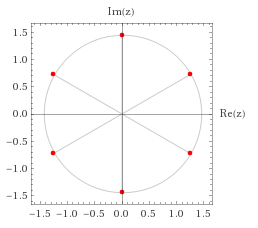
\includegraphics[scale=0.75]{sixthRoots}		
	\end{figure}
	
\section*{1.20} 
Use proposition 1.3 to derive the triple angle formulas. 
	\begin{align*}
		e^{i3\phi} &= \Big(e^{i\phi}\Big)^3 = \cos3\phi + i \sin3\phi \\  
			&= (\cos\phi + i \sin\phi)^3 \\ 
			&= (\cos\phi + i \sin\phi) (\cos\phi + i \sin\phi) (\cos\phi + i \sin\phi)\\
			&=(\cos\phi + i \sin\phi)(\cos^2\phi-\sin^2\phi+i2\sin\phi\cos\phi)\\ 
			&= (\cos^3\phi-\cos\phi\sin^2\phi-2\sin^2\phi\cos\phi) +i(2\sin\phi\cos^2\phi+\sin\phi\cos^\phi-\sin^3\phi) \\ 
		\Rightarrow \cos3\phi &= \cos^3\phi - 3\cos\phi\sin^2\phi \\ 
			\sin3\phi &= 3\sin\phi\cos^2\phi - \sin^3\phi 
	\end{align*}
	
	
\section*{1.23ae} 
Sketch the following sets in the $\mathbb{C}$ plane. \\ 

\noindent(a) $\{z\in\mathbb{C}:|z-1+i|=2\}$\\

\noindent From proposition 1.2 this set is all of the points in $\mathbb{C}$ that are of a constant distance 2 from the point $1-i$. Thus this set is a circle of radius 2 centered around $1-i$. See the following diagram. \\ 

\pagebreak 

\noindent(b) $\{ z \in \mathbb{C}: |z|=|z+1| \}$ \\

First let $z=x+iy$. Then from the definition of the set we have that: 
	\begin{align*}
		|x+iy| &= |x+iy 1| \\ 
		|x+iy|^2 &= |(x+1)+iy|^2 \\ 
		\Rightarrow x^2 + y^2 &= (x+1)^2 + y^2 \\ 
		x^2 &= (x+1)^2 \\ 
		x^2 &= x^2 + 2x + 1 \\ 
		0 &= 2x + 1 \\ 
		x &= -\frac{1}{2} 
	\end{align*}


\noindent Thus we can rewrite this set as $\{z=x+iy \in \mathbb{C} : x = -1/2\}$. Therefore the image of this set in the complex plane is a vertical line at $x=-1/2$ 
\end{document}











































































